\section{Limit on new physics}
\label{sec:limit}

%{\bf \color{red} The numbers in this Section need to be double checked.}

\subsection{Limit on number of events}
\label{sec:limnumevents}
As discussed in Section~\ref{sec:results}, we see one event 
in the signal region, defined as SumJetPt$>$300 GeV and 
\met/$\sqrt{\rm SumJetPt}>8.5$ GeV$^{\frac{1}{2}}$.

The background prediction from the SM Monte Carlo is 1.3 events.
%, where the uncertainty comes from 
%the jet energy scale (30\%, see Section~\ref{sec:systematics}),
%the luminosity (10\%), and the lepton/trigger 
%efficiency (10\%)\footnote{Other uncertainties associated with 
%the modeling of $t\bar{t}$ in MadGraph have not been evaluated.
%The uncertainty on $pp \to \sigma(t\bar{t})$ is also not included.}.
The data driven background predictions from the ABCD method 
and the $P_T(\ell\ell)$ method are $1.3 \pm 0.8({\rm stat}) \pm 0.3({\rm syst})$ 
and $2.1 \pm 2.1({\rm stat}) \pm 0.6({\rm syst})$, respectively.

These three predictions are in good agreement with each other
and with the observation of one event in the signal region.
We calculate a Bayesian 95\% CL upper limit\cite{ref:bayes.f} 
on the number of non SM events in the signal region to be 4.1.
We have also calculated this limit using 
% a profile likelihood method
% as implemented in 
the cl95cms software\cite{ref:cl95cms}, 
and we also find 4.1.  (This is not surprising, since cl95cms
also gives baysean upper limits with a flat prior).
These limits were calculated using a background prediction of $N_{BG} = 1.4 \pm 0.8$
events, the error-weighted average of the ABCD and $P_T(\ell\ell)$ background 
predictions.  The upper limit is not very sensitive to the choice of
$N_{BG}$ and its uncertainty.

To get a feeling for the sensitivity of this search to some
popular SUSY models, we remind the reader of the number of expected
LM0 and LM1 events from Table~\ref{tab:sigcont}: $8.6 \pm 1.6$ 
events and $3.6 \pm 0.5$ events respectively, where the uncertainties
are from energy scale (Section~\ref{sec:systematics}), luminosity,
and lepton efficiency.


\subsection{Outreach}
\label{sec:outreach}
Conveying additional useful information about the results of
a generic ``signature-based'' search such as the one described
in this note is a difficult issue.  
Here we attempt to present our result in the most general 
way.

Models of new physics in the dilepton final state 
can be confronted in an approximate way by simple 
generator-level studies that 
compare the expected number of events in 34.0~pb$^{-1}$
with our upper limit of 4.1 events.  The key ingredients
of such studies are the kinematical cuts described 
in this note, the lepton efficiencies, and the detector
responses for SumJetPt and \met/$\sqrt{\rm SumJetPt}$.
The muon identification efficiency is $\approx 95\%$;
the electron identification efficiency varies from $\approx$ 63\% at 
$P_T = 10$ GeV to 91\% for $P_T > 30$ GeV.  The isolation
efficiency in top events varies from $\approx 83\%$ (muons)
and $\approx 89\%$ (electrons) at $P_T=10$ GeV to 
$\approx 95\%$ for $P_T>60$ GeV. 
%{\bf \color{red} The following numbers were derived from Fall 10 samples. } 
The average detector 
responses for SumJetPt and $\met/\sqrt{\rm SumJetPt}$ are 
$1.02 \pm 0.05$ and $0.94 \pm 0.05$ respectively, where
the uncertainties are from the jet energy scale uncertainty.
The experimental resolutions on these quantities are 11\% and 
16\% respectively.

To justify the statements in the previous paragraph 
about the detector responses, we plot 
in Figure~\ref{fig:response} the average response for 
SumJetPt and \met/$\sqrt{\rm SumJetPt}$ in MC, as well as the
efficiency for the cuts on these quantities used in defining the
signal region.
% (SumJetPt $>$ 300 GeV and \met/$\sqrt{\rm SumJetPt} > 8.5$
% Gev$^{\frac{1}{2}}$).  
%{\bf \color{red} The following numbers were derived from Fall10 samples }
We find that the average SumJetPt response 
in the Monte Carlo is about 1.02, with an RMS of order 11\% while
the response of \met/$\sqrt{\rm SumJetPt}$ is approximately 0.94 with an
RMS of 16\%.

%Using this information as well as the kinematical
%cuts described in Section~\ref{sec:eventSel} and the lepton efficiencies
%of Figures~\ref{fig:effttbar}, one should be able to confront
%any existing or future model via a relatively simple generator 
%level study by comparing the expected number of events in 35 pb$^{-1}$
%with our upper limit of 4.1 events.

\begin{figure}[tbh]
\begin{center}
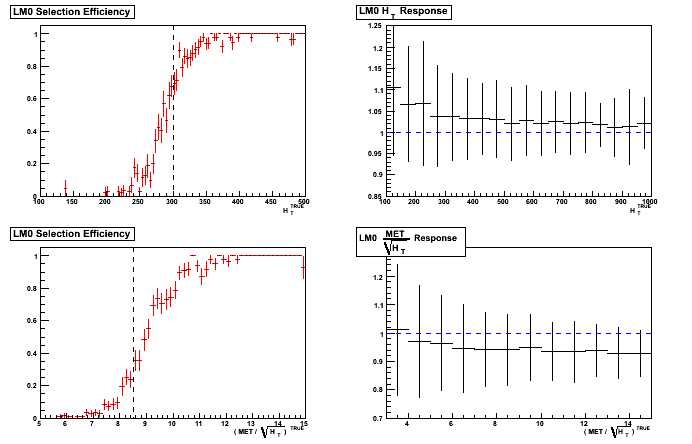
\includegraphics[width=\linewidth]{selectionEffDec10.png}
\caption{\label{fig:response} Left plots: the efficiencies
as a function of the true quantities for the SumJetPt (top) and
tcMET/$\sqrt{\rm SumJetPt}$ (bottom) requirements for the signal 
region as a function of their true values.  The value of the 
cuts is indicated by the vertical line.
Right plots: The average response and its RMS for the SumJetPt
(top) and tcMET/$\sqrt{\rm SumJetPt}$ (bottom) measurements.
The response is defined as the ratio of the reconstructed quantity
to the true quantity in MC.  These plots are done using the LM0
Monte Carlo, but they are not expected to depend strongly on 
the underlying physics.
%{\bf \color{red} These plots were made with Fall10 samples. } 
}
\end{center}
\end{figure}



%%%  Nominal
% ----------------------------------------- 
% observed events                         1
% relative error on acceptance        0.000
% expected background                 1.400
% absolute error on background        0.770
% desired confidence level             0.95
% integration upper limit             30.00
% integration step size              0.0100
% ----------------------------------------- 
% Are the above correct? y
%    1  16.685     0.29375E-06
%
% limit: less than     4.112 signal events 



%%%  Add 20% acceptance uncertainty based on LM0
% ----------------------------------------- 
% observed events                         1
% relative error on acceptance        0.200
% expected background                 1.400
% absolute error on background        0.770
% desired confidence level             0.95
% integration upper limit             30.00
% integration step size              0.0100
% ----------------------------------------- 
% Are the above correct? y
%    1  29.995     0.50457E-06
%
% limit: less than     4.689 signal events 



\subsection{mSUGRA scan}
\label{sec:mSUGRA}
We also perform a scan of the mSUGRA parameter space, as recomended
by the SUSY group convenors\cite{ref:scan}.
The goal of the scan is to determine an exclusion region in the 
$m_0$ vs. $m_{1/2}$ plane for
$\tan\beta=3$, 
sign of $\mu = +$, and $A_{0}=0$~GeV.  This scan is based on events
generated with FastSim.

The first order of business is to verify that results using
Fastsim and Fullsim are compatible.  To this end we compare the
expected yield for the LM1 point in FullSim (3.56 $\pm$ 0.06) and
FastSim (3.29 $\pm$ 0.27), where the uncertainties are statistical only.
These two numbers are in agreement, which gives us confidence in
using FastSim for this study.

The FastSim events are generated with different values of $m_0$
and $m_{1/2}$ in steps of 10 GeV.  For each point in the 
$m_0$ vs. $m_{1/2}$ plane, we compute the expected number of
events at NLO.  We then also calculate an upper limit $N_{UL}$
using cl95cms at each point using the following inputs:
\begin{itemize} 
\item Number of BG events = 1.40 $\pm$ 0.77
\item Luminosity uncertainty = 11\%
\item The acceptance uncertainty is calculated at each point
as the quadrature sum of
\begin{itemize}
\item The uncertainty due to JES for that point, as calculated 
using the method described in Section~\ref{sec:systematics}
\item A 5\% uncertainty due to lepton efficiencies
\item An uncertaity on the NLO cross-section obtained by varying the 
factorization and renormalization scale by a factor of two\cite{ref:sanjay}. 
\item A 13\% PDF uncertainty on the product of cross-section and acceptance.
This uncertainty was calculated using the method of Reference~\cite{ref:pdf} for a
number of points in the $m_0$ vs. $m_{1/2}$ plane, and was found to be 
approximately independent of mSUGRA parameters, see Table~\ref{tab:pdf}.
\end{itemize}
\item We use the ``log-normal'' model for the nuisance parameters
in cl95cms
\end{itemize}
We actually calculate three different values of $N_{UL}$:
\begin{enumerate}
\item Observed $N_{UL}$ asssuming the NLO cross-section.
\item Observed $N_{UL}$ asssuming the LO cross-section. In this case 
uncertainties due to PDFs and renormlization/factorization scales are not 
included.
\item Expected $N_{UL}$ sssuming the NLO cross-section.  This is 
calculated using the the CLA function also available in cl95cms.
\end{enumerate}

\begin{table}[hbt]
\begin{center}
\caption{\label{tab:pdf} PDF uncertainties on the product of 
cross-section and acceptance for a number of representative points
in the mSUGRA plane.}
\begin{tabular}{c|c|c|c|c|c}
$\tan\beta$ & $m_0$ & $m_{1/2}$ & sign of $\mu$ & $A_0$ & uncertanity (\%)   \\ \hline
3           & 50    & 260       & +             &  0    & $^{+13}_{-9}$ \\
3           & 50    & 270       & +             &  0    & $^{+13}_{-9}$ \\
3           & 60    & 260       & +             &  0    & $^{+14}_{-9}$ \\
3           & 200   & 200       & +             &  0    & $^{+12}_{-9}$ \\
3           & 200   & 210       & +             &  0    & $^{+13}_{-10}$ \\
3           & 210   & 200       & +             &  0    & $^{+11}_{-8}$ \\
3           & 200   & 140       & +             &  0    & $^{+16}_{-12}$ \\
3           & 140   & 150       & +             &  0    & $^{+08}_{-8}$ \\
3           & 150   & 140       & +             &  0    & $^{+14}_{-10}$ \\
10          & 60    & 260       & +             &  0    & $^{+16}_{-11}$ \\
10          & 100   & 260       & +             &  0    & $^{+14}_{-10}$ \\
10          & 100   & 260       & +             &  0    & $^{+12}_{-9}$ \\
10          & 90    & 260       & +             &  0    & $^{+15}_{-10}$ \\
10          & 240   & 260       & +             &  0    & $^{+10}_{-8}$ \\
10          & 240   & 260       & +             &  0    & $^{+13}_{-10}$  \\ \hline
\end{tabular}
\end{center}
\end{table}


An mSUGRA point is excluded if the resulting $N_{UL}$ is smaller
than the expected number of events.  Because of the quantization 
of the available MC points in the $m_0$ vs $m_{1/2}$ plane, the 
boundaries of the excluded region are also quantized.  The excluded points 
are shown in Figure~\ref{fig:tanbeta3raw}; in this Figure we also show
ad-hoc curves that represent the excluded regions.
In Figure~\ref{fig:msugra} we show our results compared with
results from previous experiments.


\begin{figure}[tbh]
\begin{center}
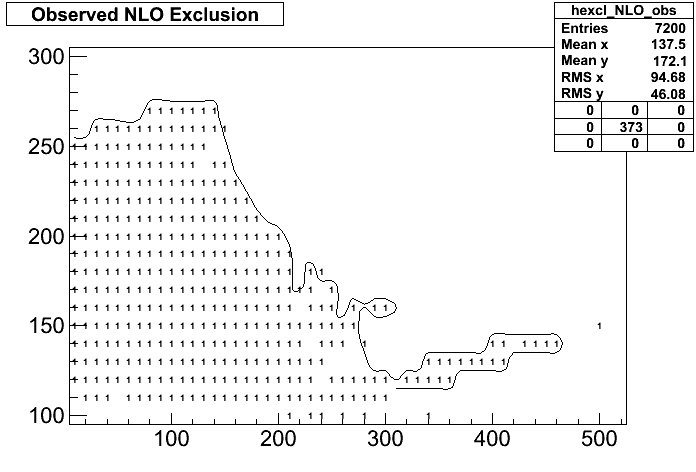
\includegraphics[width=0.4\linewidth]{tanbeta3_NLO_observed.png}
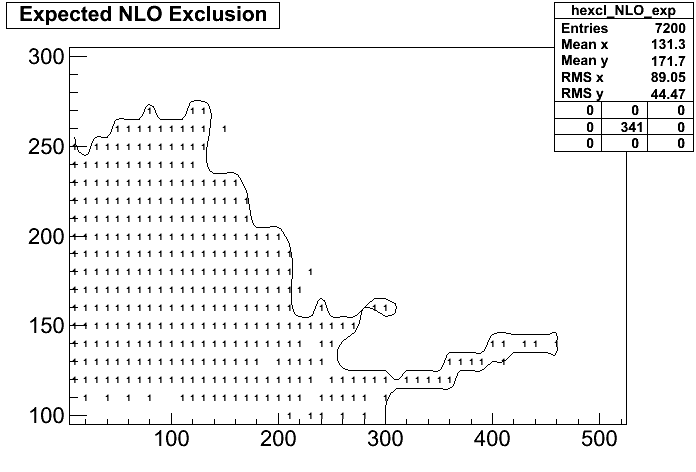
\includegraphics[width=0.4\linewidth]{tanbeta3_NLO_expected.png}
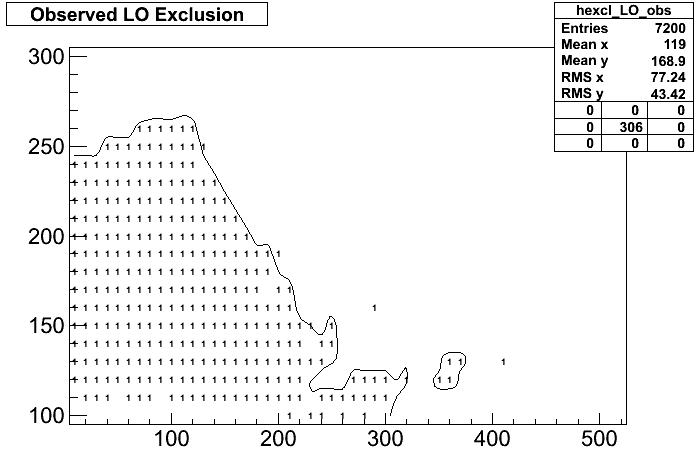
\includegraphics[width=0.4\linewidth]{tanbeta3_LO_observed.png}
\caption{\label{fig:tanbeta3raw}\protect Excluded points in the 
$m_0$ vs. $m_{1/2}$ plane for $\tan\beta=3$, sign of $\mu = +$ and $A_{0}=0$~GeVs. 
Top left: observed, using the NLO cross-section.
Top right: expected using the NLO cross-section.
Bottom left: observed, using the LO cross-section.
The curves are meant to represent the excluded regions.}
\end{center}
\end{figure}


\begin{figure}[tbh]
\begin{center}
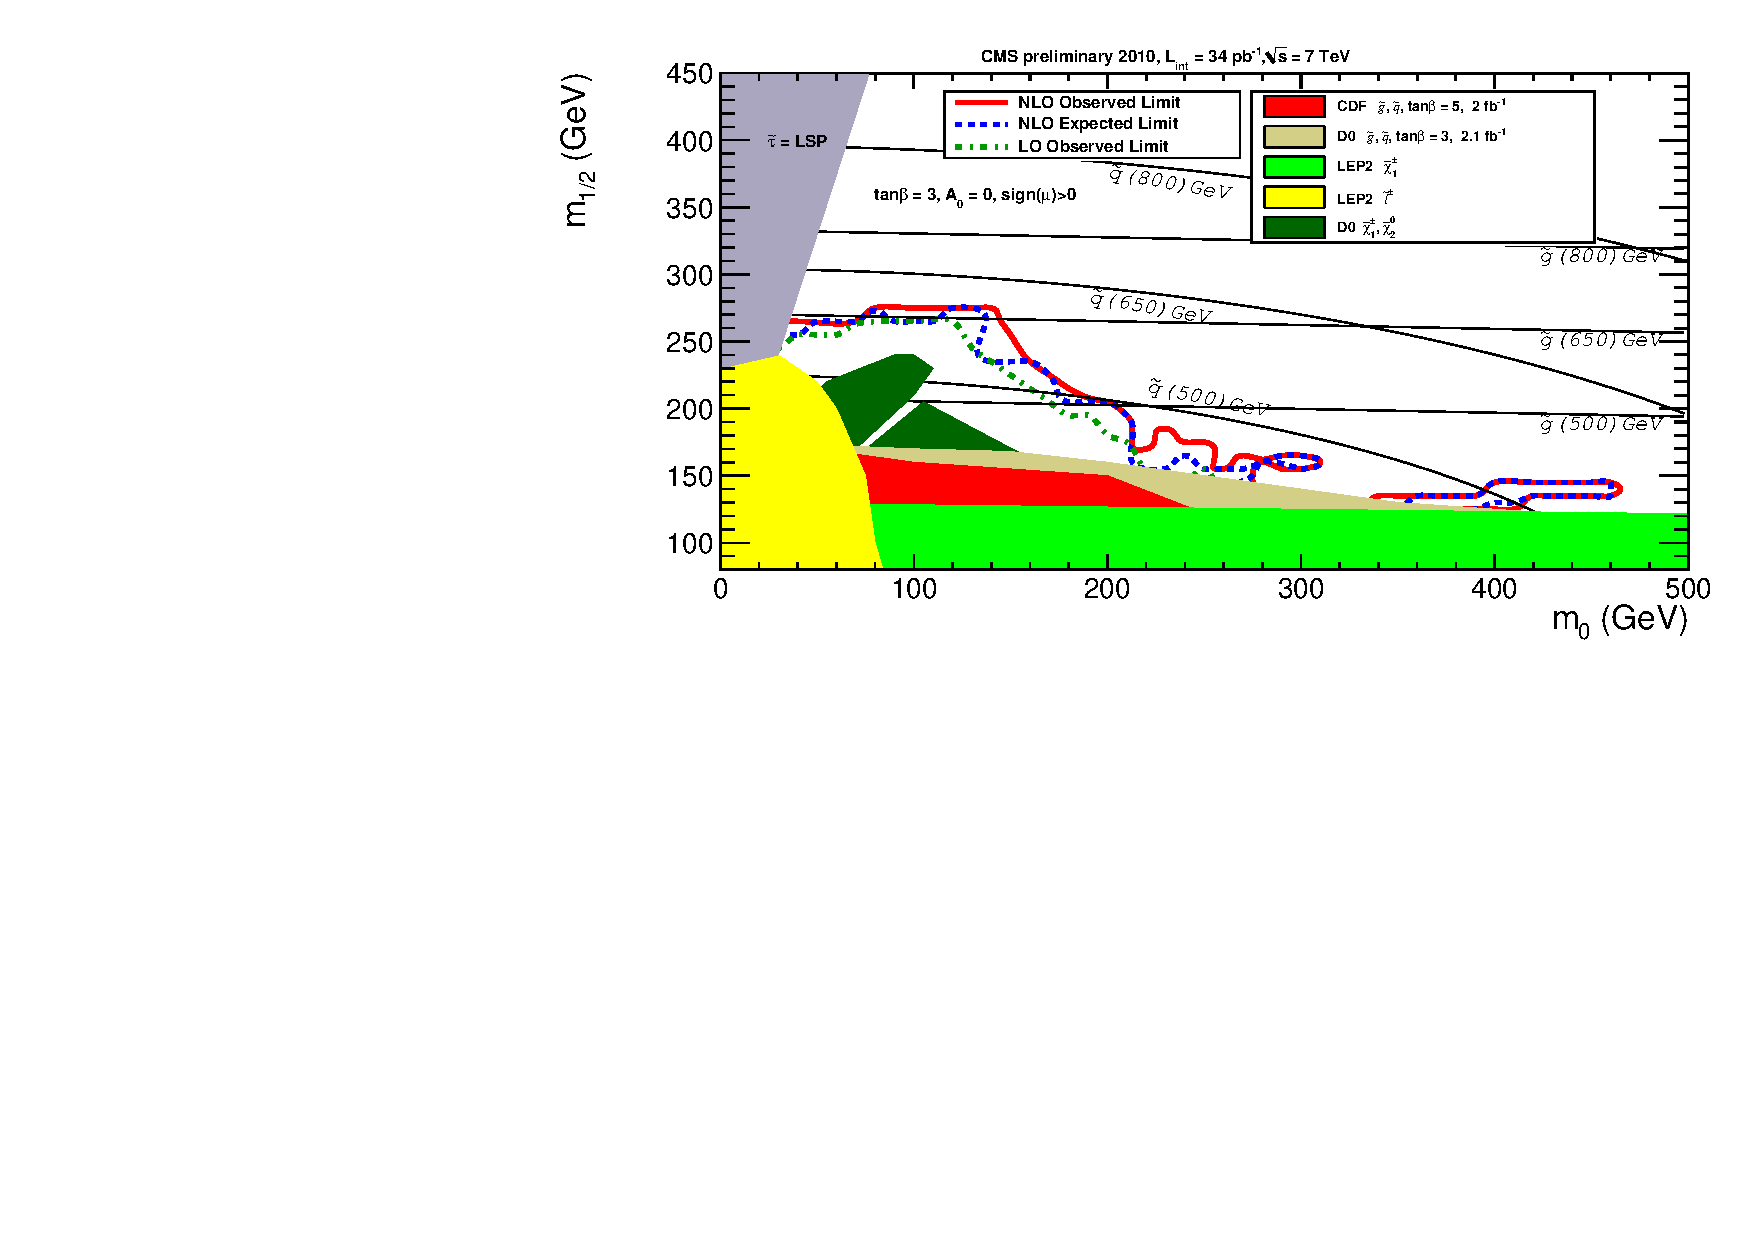
\includegraphics[width=\linewidth]{exclusion.pdf}
\caption{\label{fig:msugra}\protect Exclusion curves in the mSUGRA parameter space, 
assuming $\tan\beta=3$, sign of $\mu = +$ and $A_{0}=0$~GeVs.}  
\end{center}
\end{figure}



\clearpage

\subsubsection{Check of the nuisance parameter models}
We repeat the procedure outlined above but changing the 
lognormal nuisance parameter model to a gaussian or 
gamma-function model.  The results are shown in 
Figure~\ref{fig:nuisance}.  (In this case,
to avoid smoothing artifacts, we 
show the raw results, without smoothing).

\begin{figure}[tbh]
\begin{center}
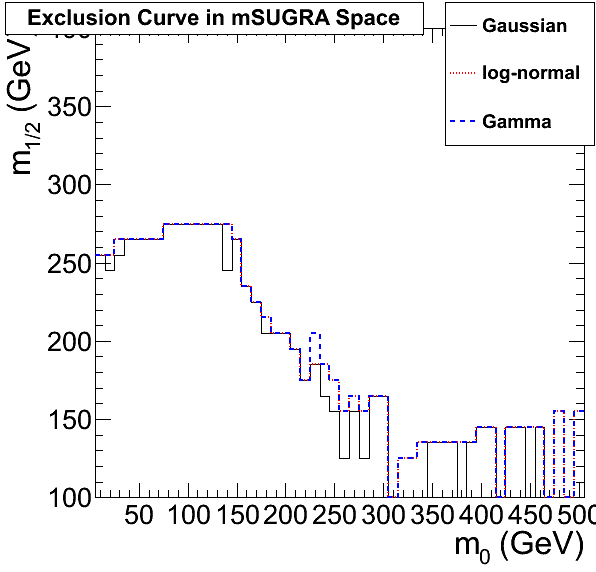
\includegraphics[width=0.5\linewidth]{nuissance.png}
\caption{\label{fig:nuisance}\protect Observed NLO exclusion curves in the 
mSUGRA parameter space, 
assuming $\tan\beta=3$, sign of $\mu = +$ and $A_{0}=0$~GeVs
using different models for the nuisance parameters. (Note: this
plot was made without the PDF uncertainties.}
\end{center}
\end{figure}

We find that different assumptions on the PDFs for the nuisance
parameters make very small differences to the set of excluded
points.
Following the recommendation of Reference~\cite{ref:cousins},
we use the lognormal nuisance parameter model as the default.


% \clearpage


\subsubsection{Effect of signal contamination}
\label{sec:contlimit}

Signal contamination could affect the limit by inflating the 
background expectation.  In our case we see no evidence of signal
contamination, within statistics.
The yields in the control regions  
$A$, $B$, and $C$ (Table~\ref{tab:datayield}) are just 
as expected in the SM, and the check 
of the $P_T(\ell \ell)$ method in the control region is
also consistent with expectations (Table~\ref{tab:victory}).
Since we have two data driven methods, with different 
signal contamination issues, giving consistent
results that are in agreement with the SM, we 
argue for not making any correction to our procedure
because of signal contamination.  In some sense this would 
be equivalent to using the SM background prediction, and using 
the data driven methods as confirmations of that prediction.

Nevertheless, here we explore the possible effect of 
signal contamination.  The procedure suggested to us
for the ABCD method is to modify the 
ABCD background prediction from $A_D \cdot C_D/B_D$ to
$(A_D-A_S) \cdot (C_D-C_S) / (B_D - B_S)$, where the 
subscripts $D$ and $S$ refer to the number of observed data
events and expected SUSY events, respectively, in a given region. 
We then recalculate $N_{UL}$ at each point using this modified
ABCD background estimation.  For simplicity we ignore
information from the $P_T(\ell \ell)$
background estimation.  This is conservative, since
the $P_T(\ell\ell)$ background estimation happens to
be numerically larger than the one from ABCD. 

Note, however, that in some cases this procedure is 
nonsensical.  For example, take LM0 as a SUSY 
point.  In region $C$ we have a SM prediction of 5.1
events and $C_D = 4$ in agreement with the Standard Model,
see Table~\ref{tab:datayield}.  From the LM0 Monte Carlo,
we find $C_S = 8.6$ events.   Thus, including information
on $C_D$ and $C_S$ should {\bf strengthen} the limit, since there
is clearly a deficit of events in the $C$ region in the 
LM0 hypothesis.  Instead, we now get a negative ABCD 
BG prediction (which is nonsense, so we set it to zero),
and therefore a weaker limit.




\begin{figure}[tbh]
\begin{center}
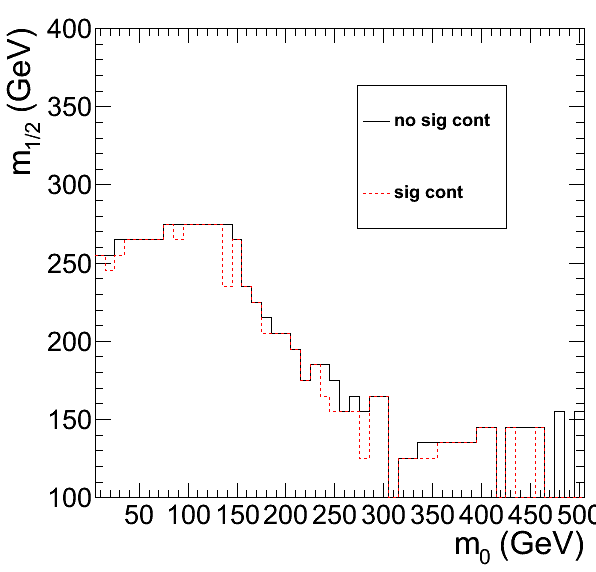
\includegraphics[width=0.5\linewidth]{sigcont.png}
\caption{\label{fig:sigcont}\protect Observed NLO exclusion curves in the 
mSUGRA parameter space, 
assuming $\tan\beta=3$, sign of $\mu = +$ and $A_{0}=0$~GeVs
with and without the effects of signal contamination.
Note: PDF uncertainties are not included.}  
\end{center}
\end{figure}

A comparison of the exclusion region with and without
signal contamination is shown in Figure~\ref{fig:sigcont}
(with no smoothing).  The effect of signal contamination is 
small, of the same order as the quantization of the scan.


\subsubsection{mSUGRA scans with different values of tan$\beta$}
\label{sec:tanbetascan}

For completeness, we also show the exclusion region calculated
using $\tan\beta = 10$ (Figure~\ref{fig:msugratb10}).


\begin{figure}[tbh]
\begin{center}
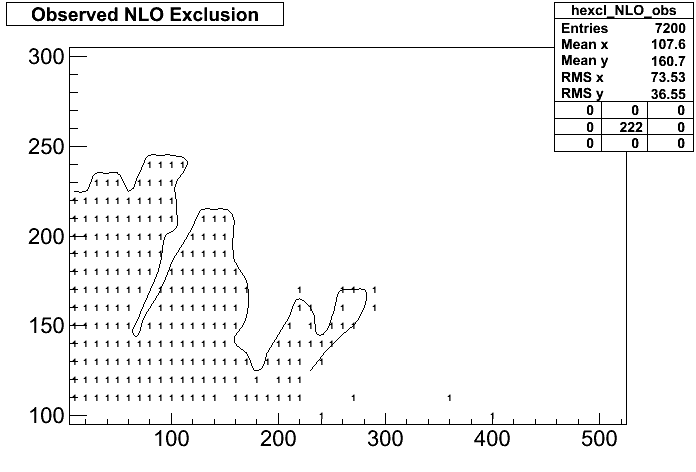
\includegraphics[width=0.4\linewidth]{tanbeta10_NLO_observed.png}
\caption{\label{fig:tanbeta10raw}\protect Excluded points in the 
$m_0$ vs. $m_{1/2}$ plane for $\tan\beta=10$, sign of $\mu = +$ and $A_{0}=0$~GeVs. 
This plot is made using the NLO cross-sections.
The curves is meant to represent the excluded region.}
\end{center}
\end{figure}

\begin{figure}[tbh]
\begin{center}
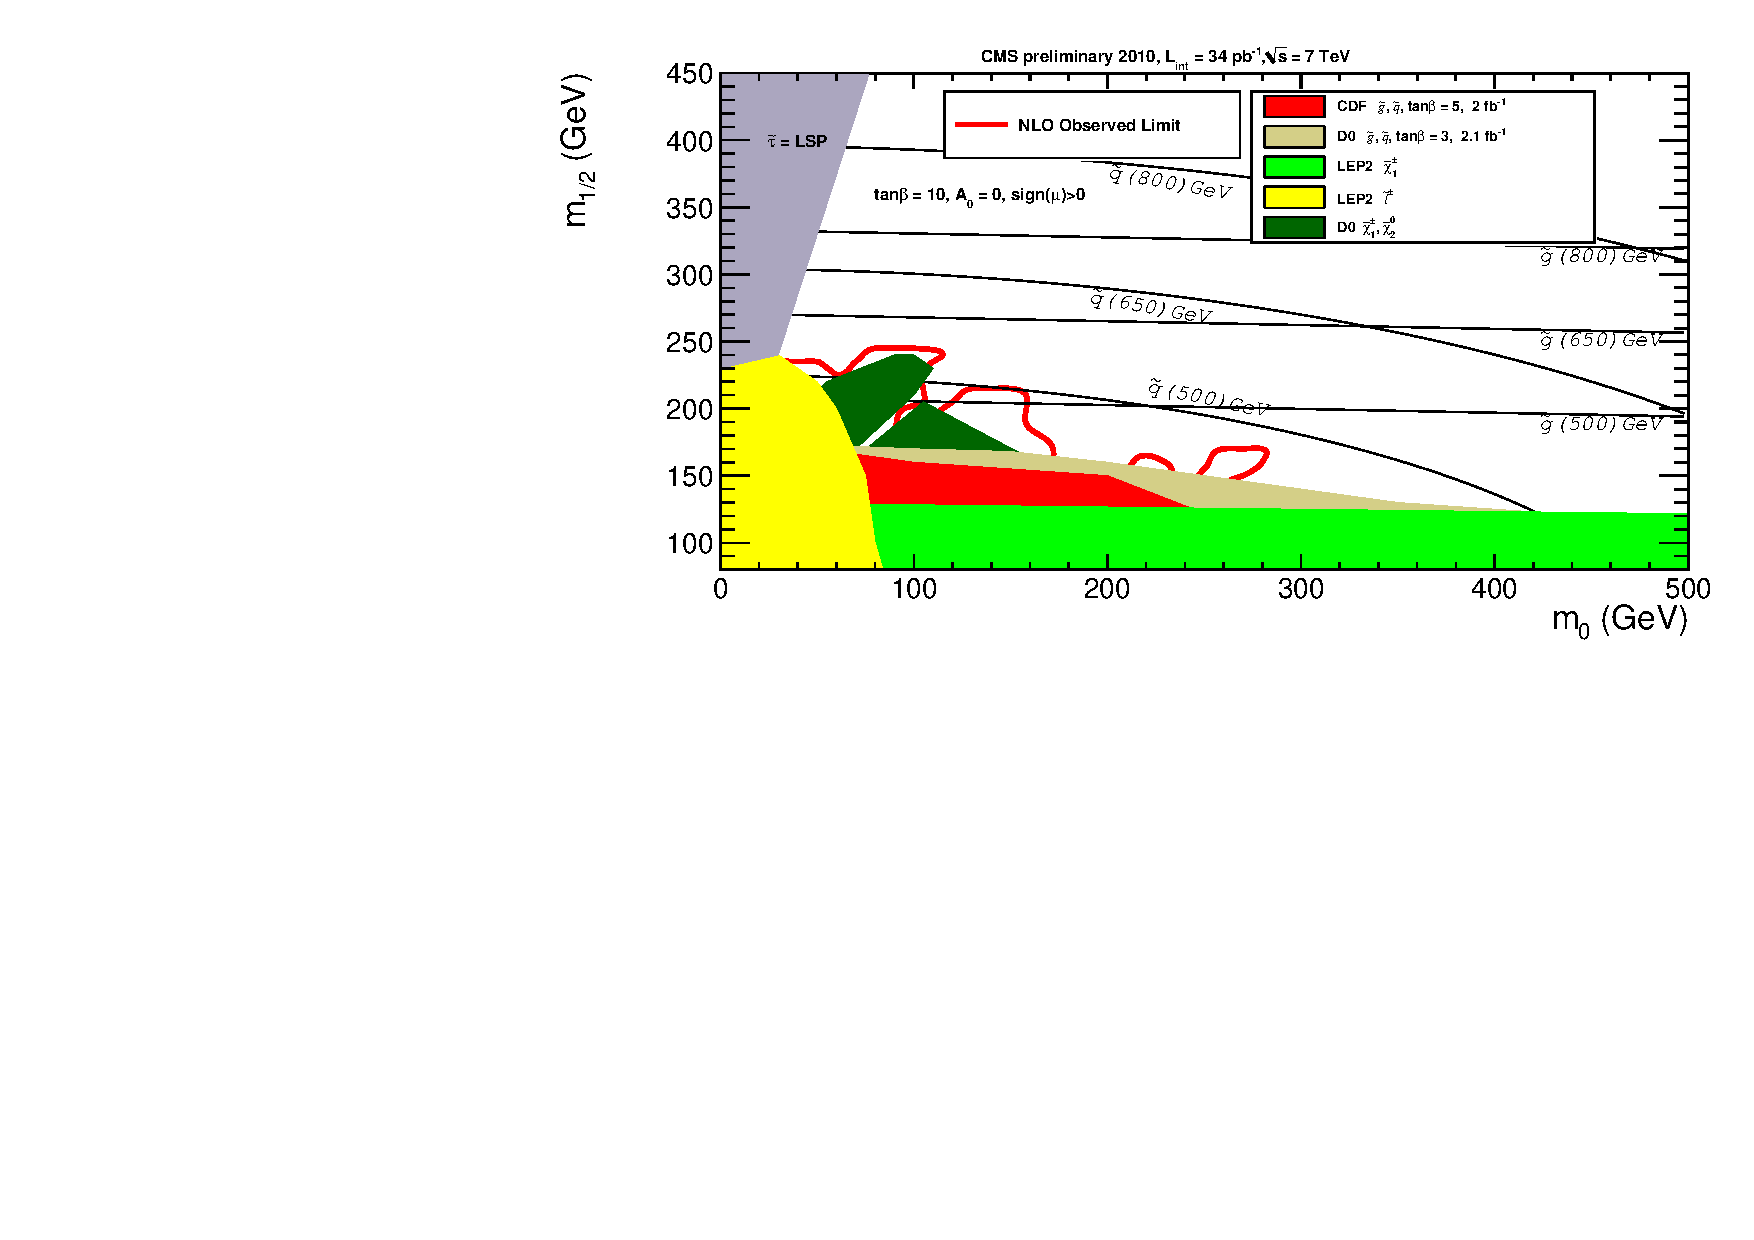
\includegraphics[width=\linewidth]{exclusion_tanbeta10.pdf}
\caption{\label{fig:msugratb10}\protect Exclusion curve in the mSUGRA parameter space, 
assuming $\tan\beta=10$, sign of $\mu = +$ and $A_{0}=0$~GeVs.}  
\end{center}
\end{figure}






